\chapter{Approach and Implementation}
\label{ch:approach}
In this chapter the basic work flow is described in detail. The process is mainly drive by an exploratory approach, but follows primarily Farines and Whiteheads~\cite{farine2015constructing} primary steps and key considerations for social network analysis to non-human animal data. The adapted and resulting process is visualized in figure~\ref{fig:process}.

The dataset was first analysed regarding data quality and to form an understanding of the dataset and behaviour of bees in general. Those findings were used to define nodes and infer associations to build the network, respectively derive parameters for the network pipeline. The static and temporal networks are analysed using network scienc tools and methods. For testing hypothesis the networks are combined with spatial and age information. Each step is explained within the following sections.

\begin{figure}[htb]
	\centering
	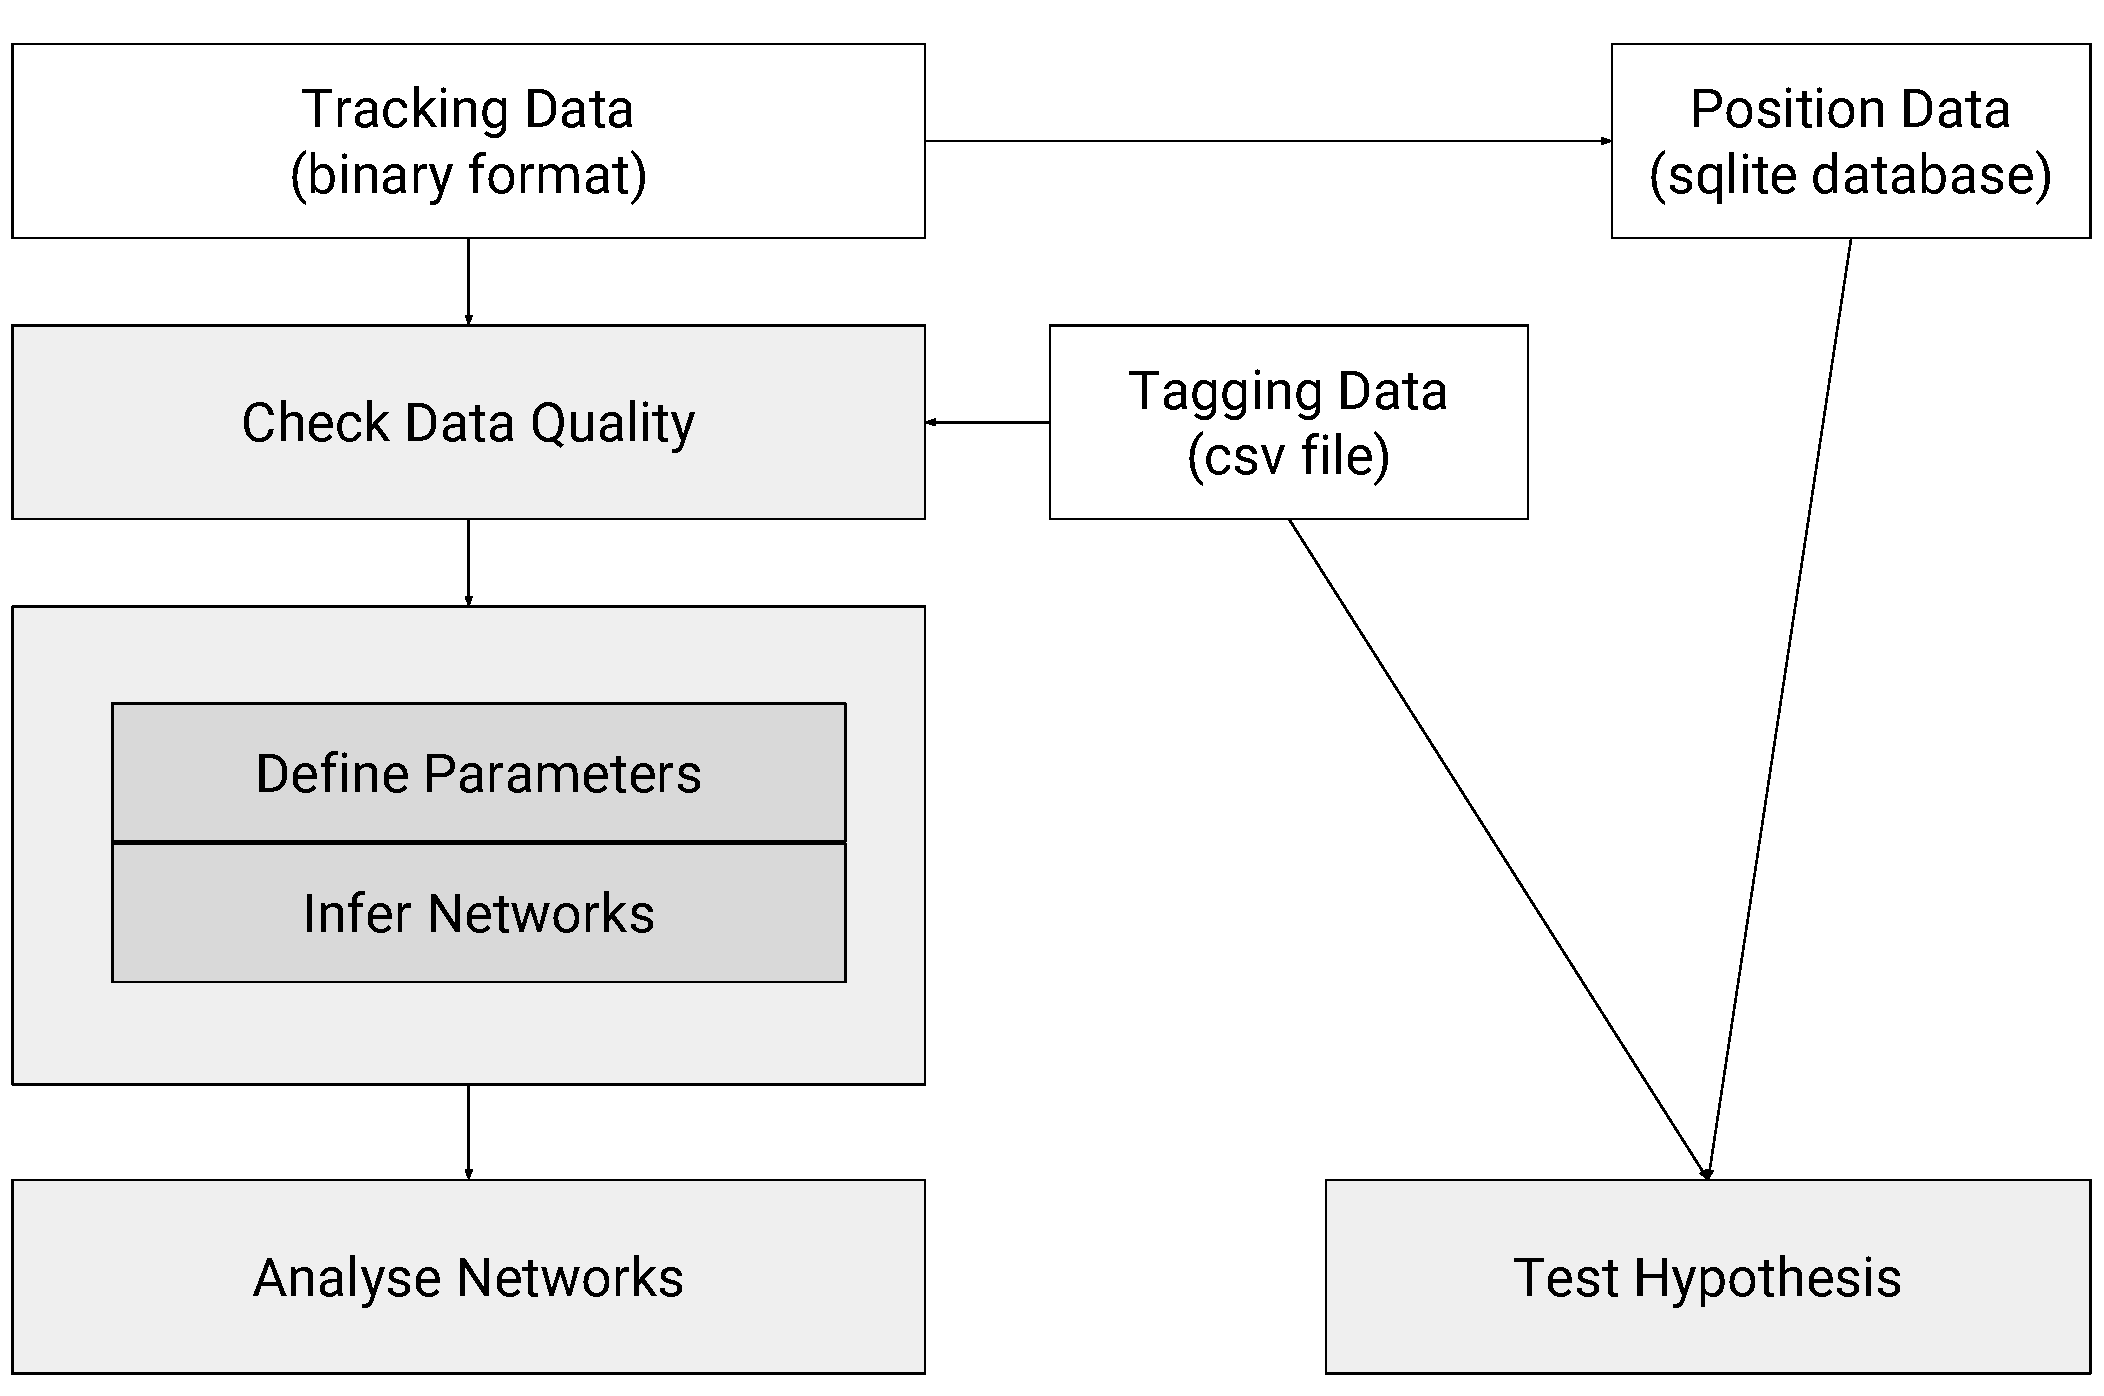
\includegraphics[width=1.0\textwidth]{Figures/process}
	\caption{Steps of the Research Approach}
	\label{fig:process}
\end{figure}


\section{The Dataset}
\label{sec:dataset}

\begin{figure}[htb]
	\centering
	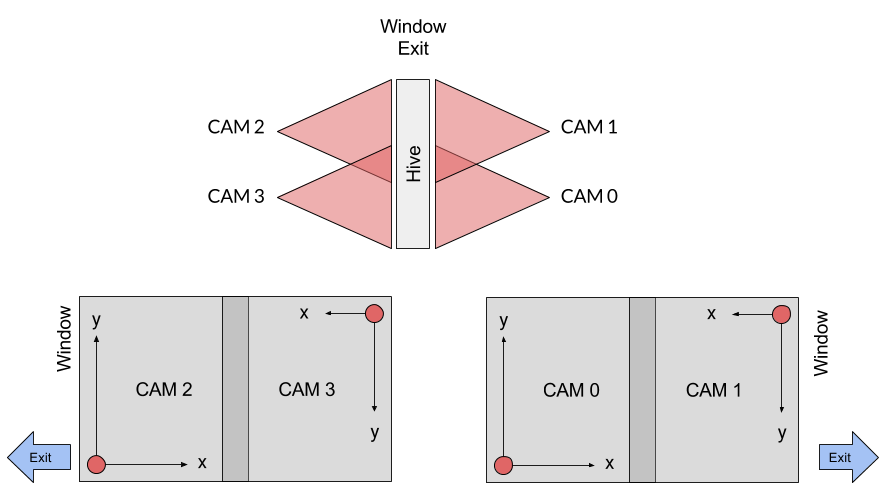
\includegraphics[width=1.0\textwidth]{Figures/setupCams}
	\caption{Camera Setup in 2016: (1) Top View:  vertical hive with two cameras for each side, overlapping in the middle. (2) Front View: left and right camera setup, the red dot indicated the origin $(0,0)$ of the camera.}
	\label{fig:cams}
\end{figure}

\begin{figure}[htb]
	\centering
	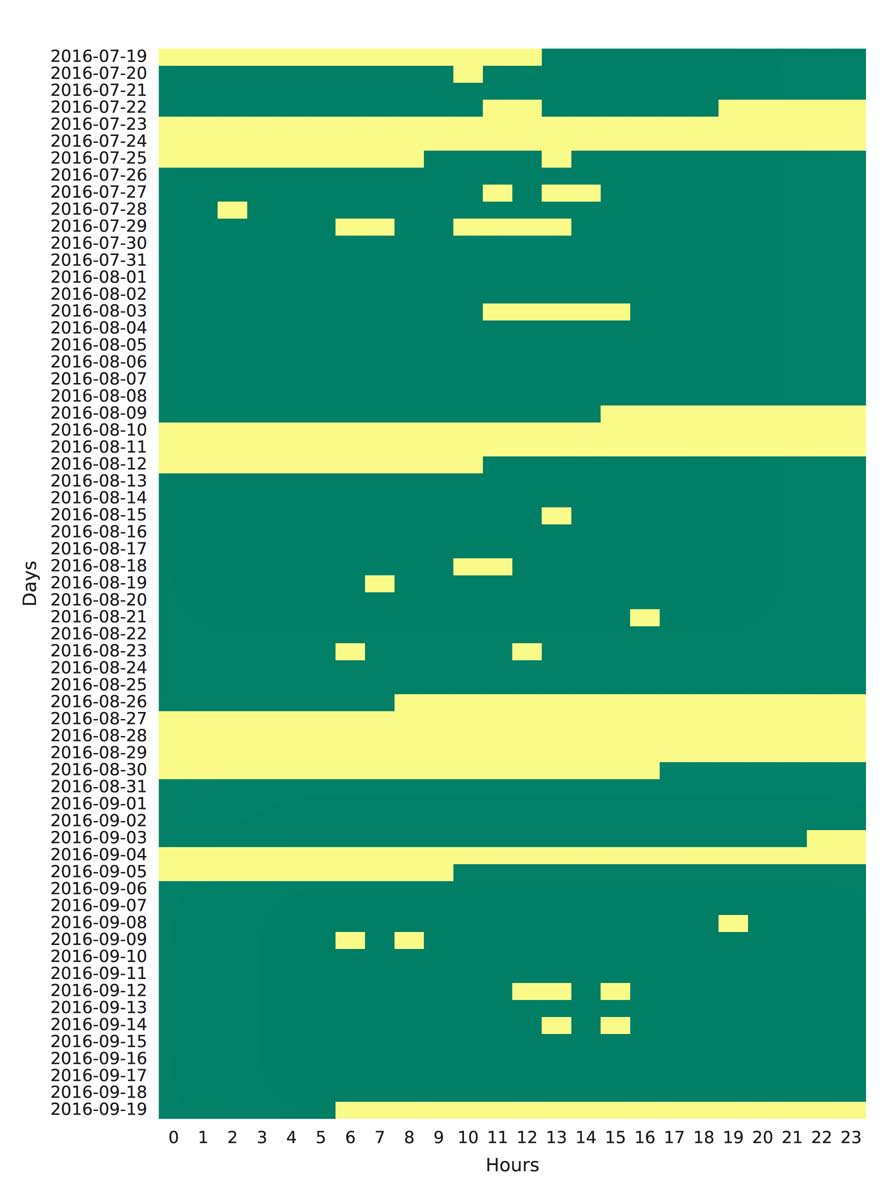
\includegraphics[width=0.6\textwidth]{Figures/recording}
	\caption[Recording Season]{Recording Season with maintainance and failures: \emph{Yellow} indicates recording went without any big interruption; \emph{Green} indicates maintainance work or technical failures of one or all cameras. This is calculated using the expected number of files produced by each camera per hour.}
	\label{fig:period}
\end{figure}

The basis of the dataset are video files, that capture tagged honey bees of one colony in a two sided observation hive.
Each individual of the colony, including about 3200 bees, were tagged with circular 12-bit markers. Four cameras were used to film the hive, the setup of the cameras is illustrated in figure~\ref{fig:cams} and an example of tagged bees is shown in section~\ref{ch:intro}, figure~\ref{fig:markers}.

\begin{figure}[htb]
	\centering
	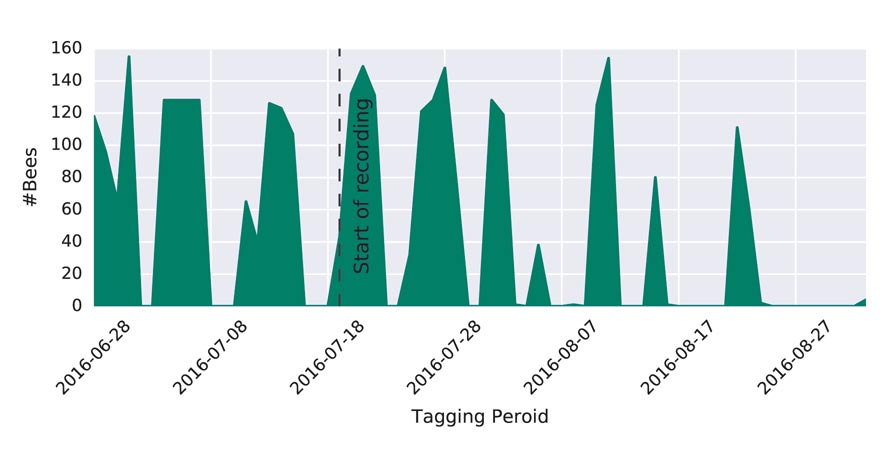
\includegraphics[width=1.0\textwidth]{Figures/tagging_period}
	\caption[Tagging Frequency]{Tagging frequency of bees: The bees were primarily tagged during the week. On average 48 bees were tagged each day, considering only tagging days, the average is about 91 ($\pm50$) bees (median 118).}
	\label{fig:tagging}
\end{figure}

The recording season lastet nine weeks (63 days), around the clock, from 19.07.2016 until 19.09.2016, with some interruptions due to maintainance and technical failures (figure~\ref{fig:period}). The recording resolution of each camera is three frames per second, aiming for $1024$ frames (about $5.7$ minutes) for a video files. For each frame, bee detections were extracted by using an image analysis pipeline, which is explained in detail in~\cite{wario2015automatic}. The resulting detection data is stored in a binary file format.
A python library called \emph{bb-binary}\footnote{\url{https://github.com/BioroboticsLab/bb_binary}; Last accesed: 2106-02-16, 04:28PM} provides easy access to the binary files. Each file in bb\_binary file format corresponds to a video file of a single camera.
The size of the complete dataset for 2016 is $470$~GB, about $7.5$~GB of binary data per day.

Exactly $3.191$ bees were tagged. The tagging period is 67 days long. The tagging started on 28.06.2016 (22 days before the recording started) and lasted until 02.09.2016 (17 days before the recording ended). The young bees were tagged and then added to the hive, about noon each day. The overall tagging frequency is shown in figure~\ref{fig:tagging}. The hatching day for each bee is known, therefore the age of each bee.



\subsection{Structure of the Dataset}
The data is organised in \emph{frame container}, wich corresponds to a video file of a single camera. A frame container holds all \emph{frames} for that specific video.
Each frame has a list of all bees detected by the image analysis pipeline.
A \emph{detection} has the following attributes, which are relevant to this project:

\begin{itemize}
\item \textbf{xpos}: $x$ coordinate of bee with respect to the image in pixel
\item \textbf{ypos}: $y$ coordinate of bee with respect to the image in pixel
\item \textbf{radius}: of the circular 12-bit tag
\item \textbf{decodedId}: decoded 12-bit id, the bit probabilities are discretised to 0-255
\end{itemize}

Besides further information, the frame container specifies the camera, which took the video. A frame is also attributed with a timestamp. The data can be accessed iterating on frame container or on frame level, in both cases using two timestamp parameters for specifying the time interval. The complete data scheme can be found on github\footnote{\url{https://github.com/BioroboticsLab/bb_binary/blob/master/bb_binary/bb_binary_schema.capnp}; Last accessed: 2106-02-16, 04:46PM}. 


\subsection{Data Quality and ID Confidence}
\label{subsec:confidence}

Each bit of the decoded 12-bit ID represents a probability between $0$ and $255$. That means when using a high ID confidence\footnote{The confidence of an specific ID is the minimum of all bits-confidences.} results in less data, but with a higher accuracy.
A low confidence results in more data, but rather uncertaity and a higher error. A good tradeoff between data quality and amount of data should be chosen. Figure~\ref{fig:tradeoff} shows the proportion of wrong detections (as a fraction of all data) depending on the confidence level for all four cameras.
A confidence level of $0.95$ results in about $59\%$ of remaining data, of those about $6\%$ are wrong detections. This level of confidence is chosen.

TODO: testing weather nodes in the created network are bees, who are alive\\

\begin{figure}[htb]
	\centering
	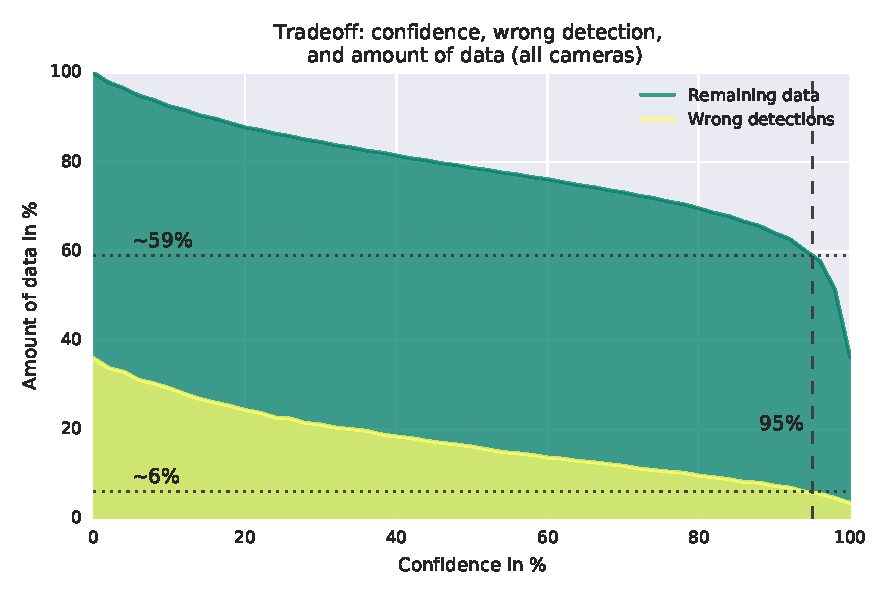
\includegraphics[width=1.0\textwidth]{Figures/tradeoff}
	\caption[Tradeoff: Confidence level, data quality and amount of data]{On 21.07.2016, about half of the bee tags were used up. This day was chosen to determine the effects of the ID confidence level on data quality and amount of remaining data. For each camera a five minute test dataset was chosen (15:00-15:05). For a sample ($n= 100.000$) of remaining detection, the age was determined, negative ages were counted as wrong detections.}
	\label{fig:tradeoff}
\end{figure}

\subsection{Influence of ID Confidence on Tracking Fragmentation}
\label{subsec:tracking}

Bee tracks are sequences of zero and ones indicating the absence and presence of bees over a specified time period. The ID confidence has also an effect on the fragmentation of bee tracks. A higher confidence level leads to more gaps in the tracks. 
The average total amount of absence time (zeros) per bee, is slightly decreasing with an increasing confidence level, because errors are filtered out (low number of 1 and the rest zeroes). The average number of fragments is increasing with an higher confidence level. That means also that the number of gaps of different sizes (e.g. 1,2,3) is increasing with a higher confidence level as well (figure~\ref{fig:fragments} and~\ref{fig:gaps}).
The absence of bees can have a lot of reasons, not only the confidence level. A bee can beinside a cell, outside the hive, not detected by camera because inside the exit, backwards on the window pane, difficult angle of tag, coverd by another bee, and so.

\begin{figure}
    \centering
    \begin{subfigure}[b]{0.45\textwidth}
        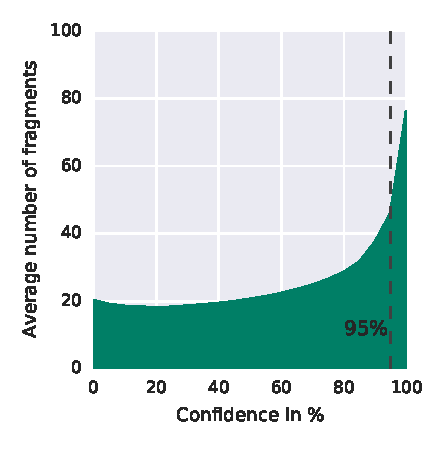
\includegraphics[width=\textwidth]{Figures/fragments}
        \caption[Average Number of Fragments]{Fragments}
        \label{fig:fragments}
    \end{subfigure}
    ~ %add desired spacing between images, e. g. ~, \quad, \qquad, \hfill etc. 
      %(or a blank line to force the subfigure onto a new line)
    \begin{subfigure}[b]{0.45\textwidth}
        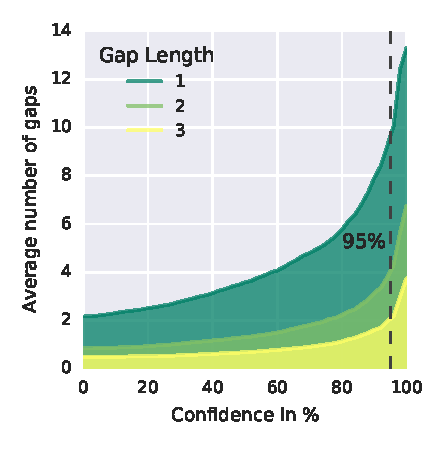
\includegraphics[width=\textwidth]{Figures/gaps}
        \caption[Average Number of Gaps]{Gaps}
        \label{fig:gaps}
    \end{subfigure}
    \caption{The higher the confidence level the higher the number of fragments and gaps of size 1, 2, and 3.}
    \label{fig:animals}
\end{figure}


\subsection{Statistical Description of the Dataset}
Maybe i will fill this part, when I need it, later.\\
speed of bees\\
presence and absence of bees (counted and as duration)\\
presence and absence of bee-pairs (counted and as duration)\\
number of detected bees per day (and hour)\\ 


\subsection{Implications}
For further analysis I use the days 30.07.2016, 31.07.2016, 01.08.2016 and 02.08.2016 with a confidence level $95\%$ [TODO: evaluate confidence level]. This period is chosen, because it is a contiguous time span close to the recording start.
Because of the high fragmentation level, the inferring of edges (bees who are close to each other at the same time), should be not that strict, or at least variable. This has to be taken into acoount, when looking at spatialy close bees.


\section{Inferring Networks}

The following part describes the pipeline for generating spatial proximity networks out of honey bee tracking data. A node in the network is a bee. They are distinguished by IDs. Only bees are in the network who interact with other bees, that means they have at least one edge and a degree of one.

Two bees are associated (spatially close to each other), if their distance is minor to a \emph{maximum distance}. As everything is very close in a bee hive this value is hard to choose. Only this criteria is very week, meaning having a resolution of three frames per seconds results in interactions which could only last for $0.33$ seconds. So an additional parameter the \emph{minimum contact duration} is introduced, it is the minimum time they have to spend at least nearby to be called associated.

Taking the fragmentation of tracks into account, it is obvious that two bees could be nearby but not at the very same time, but slightly shifted. So the minimum contact duration would be too errow prone. To overcome this issue one could correct the bee tracks, by filling gaps of varius sizes and interpolating the position of that bee accordingly. This is rather time consuming for this amount of tracking data (TODO: naja so doll auch nicht, scipy.ndimage.morphology.binary\_dilation) and also considering, that the tracking data is going to be improved in the future, then manipulating the raw data seems senseless. I rather perform a gap filling (maybe similar to binary dilation) on the time series of pairs, but not on the bee tracks, because this is independent of the input data.

To evaluate this method I compared the hemming distance of resulting bee pairs for (1) Correcting Bee Tracks (fill gaps size one), then extract pairs, (2) Bee tracks without correction, then extract pairs and (3) Bee Tracks without correction, but corrected extracted pairs (fill gaps size one). [TODO: Wie soll das Ergenis hier hin?]

\subsection{Network Pipeline}

The network pipeline takes as input a path to an bb-binary repository and outputs a graph in graphML file format. All cameras are included in the pipeline. The pipeline takes the following parameters:

\begin{itemize}
\item path to data
\item id confidence in the range 0 to 1
\item gap size in frames - size of gap, which is used to corret bee pair time series
\item maximum distance in px - maximum distance of bees (spatial proximity)
\item minimum contact duration in frames - how many frames they need to spend nearby
\item start timestamp - start of network slice
\item window size in minutes - size of time window for aggregating the network
\item number of used CPUs for parallelization
\end{itemize}

The pipeline is parallelized on frame level, that means, each process gets a portion of the data and extracts interactions, the main process, adds everything up and creates the network. The steps are the following:

\begin{enumerate}
\item For each camera: filter detections by ID confidence
\item Simple stitching of the two sides of the hive.
\item Extract close pairs.
\item Generate time series for each pair.
\item Correct pair time series.
\item Extract interactions/contacts from time series.
\end{enumerate}


\subsection{Edge weight and Thresholding}
Edges are attributed with three parameters. The first one is the frequency of contacts, so how often they share a close position. The second parameter is the total duration of contact, how many time frames in total they spend close by.
 
TODO. document what threshold for edges was used.

\subsection{Pipeline Parameters}
For performing the following network analysis, I chose the parameters as follows:

\begin{figure}
    \centering
    \begin{subfigure}[b]{0.45\textwidth}
		\centering
		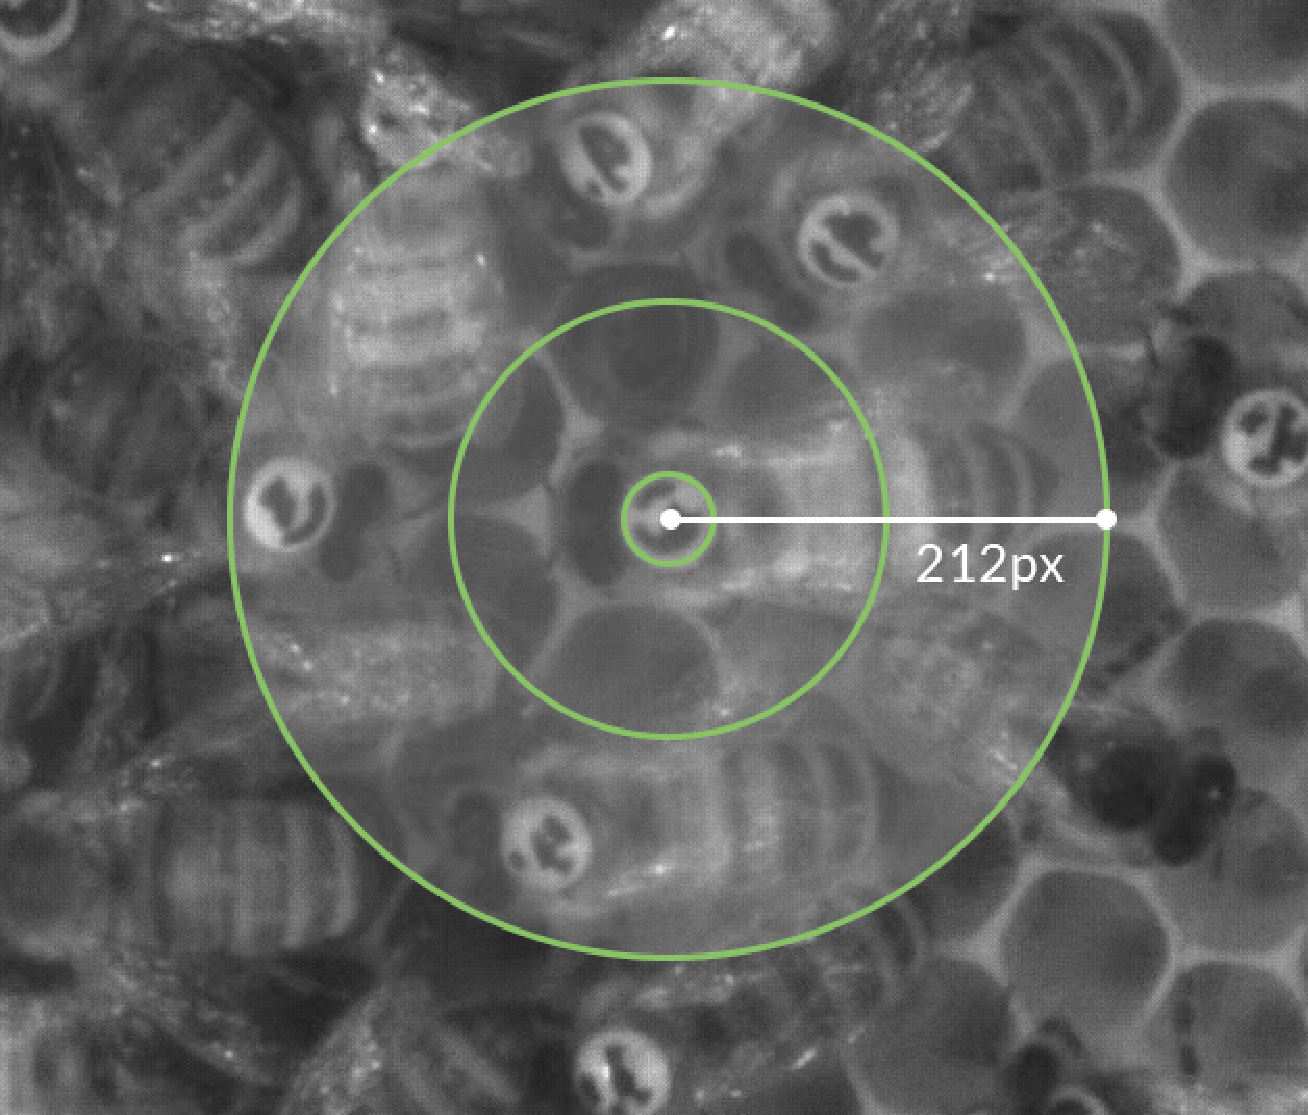
\includegraphics[width=\textwidth]{Figures/radius}
		\caption[Contact Radius]{Contact Radius}
		\label{fig:radius}
    \end{subfigure}
    ~ %add desired spacing between images, e. g. ~, \quad, \qquad, \hfill etc. 
      %(or a blank line to force the subfigure onto a new line)
    \begin{subfigure}[b]{0.45\textwidth}
	    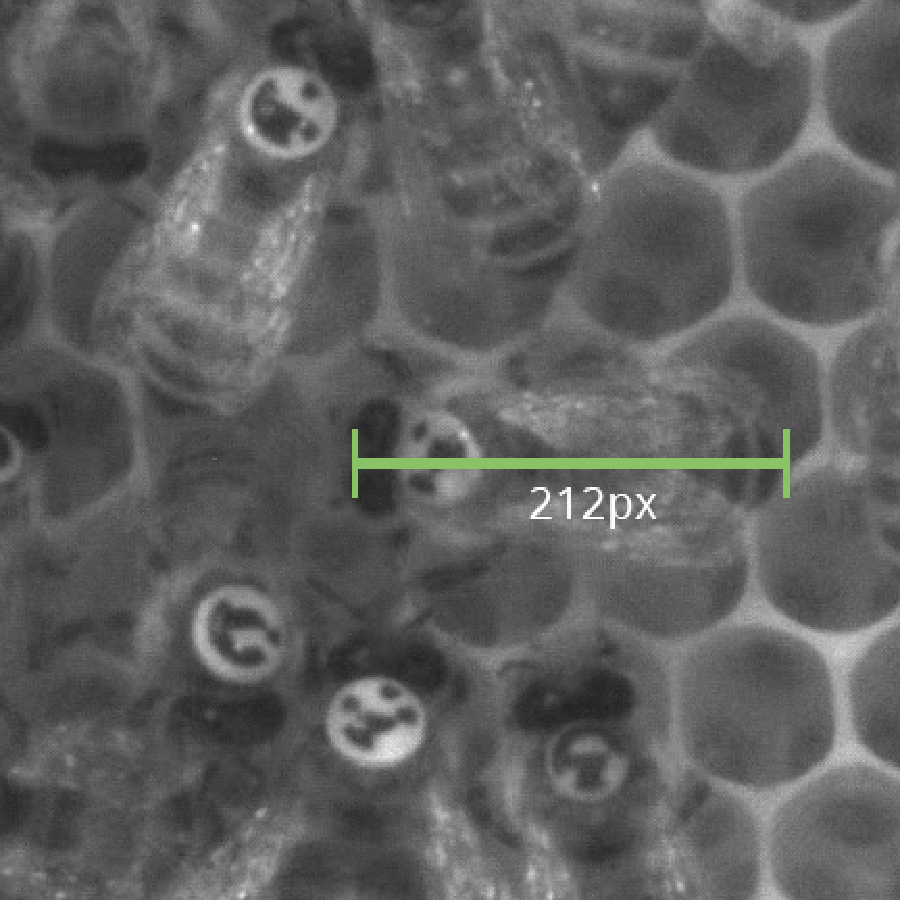
\includegraphics[width=\textwidth]{Figures/sizeTagBee}
        \caption[Bee and Tag Size]{Bee and Tag Size}
        \label{fig:size}
    \end{subfigure}
    \caption{Distance Between Bees: The average bee length is 212px, according to this, the maximal distance between bees is chosen.}
    \label{fig:contactRadius}
\end{figure}

\begin{description}
\item[Confidence] As explained in section\ref{subsec:confidence}, the confidence is set to $95\%$.

\item[Maximal Distance] I chose the length of a bee body $212$px ($\pm 16$px), according to \textcite{baracchi2014socio}, as the maximal distance between two bees (see figure~\ref{fig:radius}). The average bee length was determinded by manually measuring the length of all bees ($n=337$) in four images (one for each camera, 21.07.2016, 03:00PM) using the tool ImageJ\footnote{\url{http://imagej.net/Welcome}; Last accessed: 22.02.2016}.

\item[Minimal Contact Duration] This is set to 3 frames (one second), to exclude errors. TODO: I do not know why actually and how to justify this. \textcite{mersch2013tracking} excluded interactions below one second as well. I would rather look at the average speed of moving bees, to exclude passing bees, but then shorter interactions are excluded. Looking at the length of 1-chains of the pair time series (after filling the gaps), the mode=1, median=2 and mean=4. Three frames corresponds to 57\% of all 1-chains, seem to be reasonable. (4 = 66\%) (same dataset as in gap size)

\item[Gap Size] The gap size is set to two frames. This value corresponds to the median of gap length of bee tracks (mode=1, mean=14) and median of gap length in pair time series (mode=1, mean=27). This is tested for a 10 minute dataset for camera 1 (because it  had the most detections).
\end{description}


\section{Static and Temporal Analysis}
dataset used here 1 day and one hour of that day\\

\subsection{Static Network Analysis}
The following network properties were analysed for a static day and hour network.\\
TODO: list of properties. (similar to what others have done)

\subsection{Temporal Analysis}
consecutive day networks\\
one day split up in hours\\

\section{Attributed Data and Hypothesis Testing}
Hypothesis\\
(1) Communities reflect groups of bees working in different areas of the hive and\\
(2) Communities reflect different age groups\\

The data which was used to test the hypothesis (1) is saved in a sqlite database for faster access, because using bb\_binary (parsing the data over and over again) was to slow. For testing if lists of positions (spatial ditribution) are different the test XY was used [TODO: what to use here]

For hypothesis (2) the data is stored as a csv file of birth dates of each bee. For testing if age goups are different the Kolmogorov Smirnov Test was used.

\section{Implementation, Runtime and Complexity}
For implementing the network pipeline python, with pandas and numpy, are used, because the bb\_binary library, for accessing the tracking, data is only available in python. The networks, in graphML format, are created using the python library \emph{NetworkX}\footnote{\url{https://networkx.github.io/} ; Last accessed: 2017-02-17, 08:07PM} in version 1.11.
iGraph for community detection\\
some bash scrips for generating multiple networks\\

bottleneck is reading bb\_binary data into pandas dataframes\\
using multithreading for distribution on frame level (a process gets X frames for processing)\\

maybe some table with how long nees what with how many cores (hom much RAM and so on)\\